\chapter{Appendix: Dataset Structure and Sample Annotations}
\label{app1}

This appendix provides additional details about the datasets used in the project. The main report describes the methodology and evaluation, while this appendix summarises the common annotation format, the CO3D and UMD+GT organisations, and an example object instance.

\section{Common Annotation Format}

All experiments use a shared JSON annotation format. Each sample contains:

\begin{verbatim}
{
  "id": "cup::cup_001",
  "category": "cup",
  "instruction": "find the view where the printed design is front-facing",
  "views": [
    "E:/.../view_01.jpg",
    "E:/.../view_02.jpg",
    "E:/.../view_03.jpg",
    "E:/.../view_04.jpg",
    "E:/.../view_05.jpg"
  ],
  "gt_views": [
    "E:/.../view_01.jpg",
    "E:/.../view_05.jpg"
  ]
}
\end{verbatim}

UMD samples additionally store \texttt{affordance}, \texttt{tool}, \texttt{split}, and per-view affordance areas. The evaluation code can group results by \texttt{category} or by \texttt{affordance} and can split by object number or by an explicit \texttt{split} field.

\section{CO3D Folder Structure}

The CO3D-derived data is organised by category and object instance:

\begin{verbatim}
CO3D-subset-<category>/
    <category>/
        <category>_001/
            view_01.jpg
            view_02.jpg
            view_03.jpg
            view_04.jpg
            view_05.jpg
        <category>_002/
            ...
\end{verbatim}

Five categories are used: book, cup, handbag, remote, and teddybear. Each has 30 instances and five viewpoints. Combined annotations are stored in \texttt{E:/CO3D-combined}. The shuffled annotation file randomises both view order within each sample and sample order in the file, removing first-view bias.

\section{UMD+GT Conversion Summary}

UMD+GT source data contains turntable RGB frames and affordance masks for 104 tools. The conversion script:

\begin{itemize}
    \item extracts RGB frames only;
    \item samples five views at 20\% increments, with multiple shifted starts per tool;
    \item creates one sample per affordance present on the tool;
    \item marks ground-truth views by relative affordance area (\(\geq 80\%\) of the maximum);
    \item drops samples with no clear best view or with negligible affordance area.
\end{itemize}

The resulting annotation file contains 1{,}026 samples (603 train / 78 val / 345 test). Random-pick chance accuracy is approximately 0.43.

\section{Sample CO3D Dataset Entry}

Table~\ref{tab:sample-dataset-entry} shows an example CO3D entry.

\begin{table}[htbp]
    \centering
    \caption{Sample CO3D dataset entry for one object instance.}
    \label{tab:sample-dataset-entry}
    \begin{tabular}{ll}
        \hline
        Field & Example \\
        \hline
        Object category & \texttt{cup} \\
        Object instance & \texttt{cup\_001} \\
        Candidate views & \texttt{view\_01.jpg}--\texttt{view\_05.jpg} \\
        Instruction & \textit{find the view where the printed design is front-facing} \\
        Ground-truth views & \texttt{view\_01.jpg}, \texttt{view\_05.jpg} \\
        Evaluation budgets & \(k = 1,2,3,4,5\) \\
        \hline
    \end{tabular}
\end{table}

\section{Example of Five Candidate Viewpoints}

Figure~\ref{fig:sample-five-views} shows an example object instance with five candidate viewpoints. The active view selection system scores these views against the language instruction and selects a budgeted subset before final reranking.

\begin{figure}[htbp]
    \centering

    \begin{minipage}{0.18\textwidth}
        \centering
        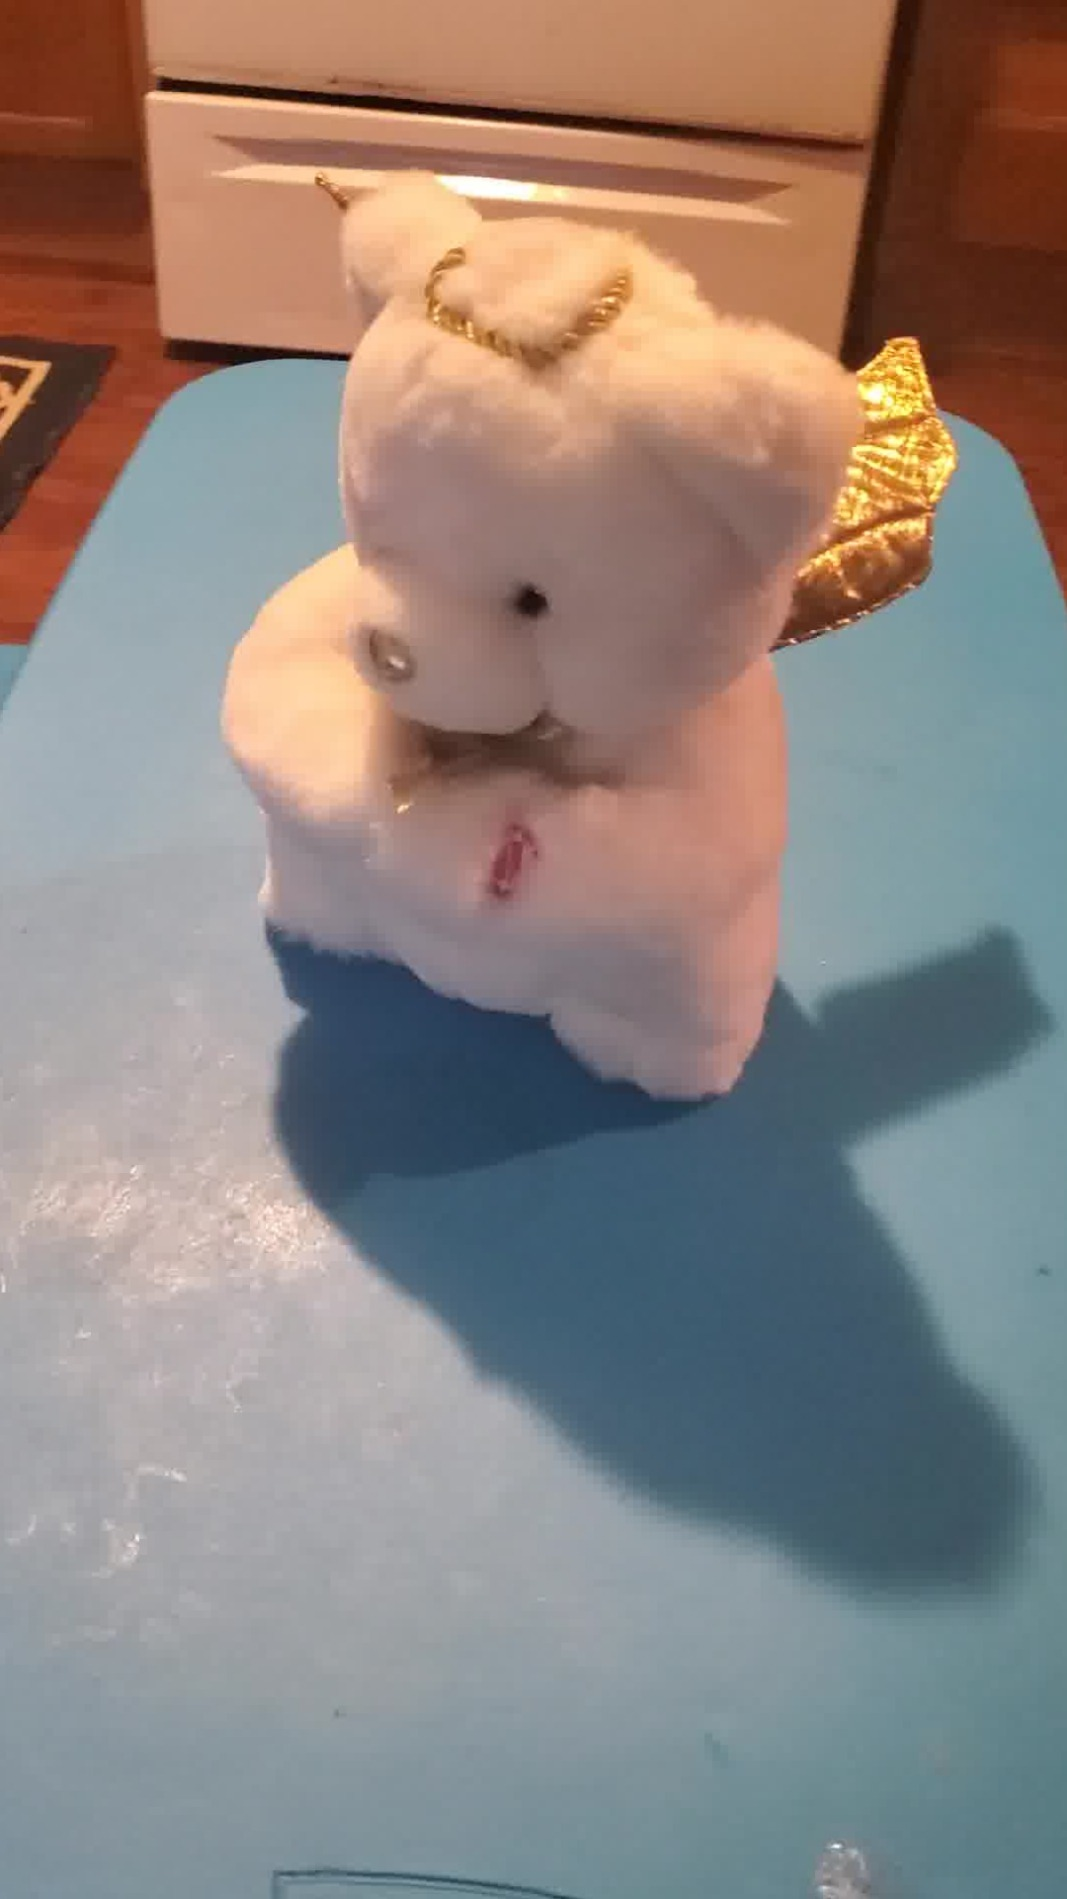
\includegraphics[width=\linewidth]{figures/sample_object/view_01.jpg}
        \vspace{2mm}
        \texttt{view\_01}
    \end{minipage}
    \hfill
    \begin{minipage}{0.18\textwidth}
        \centering
        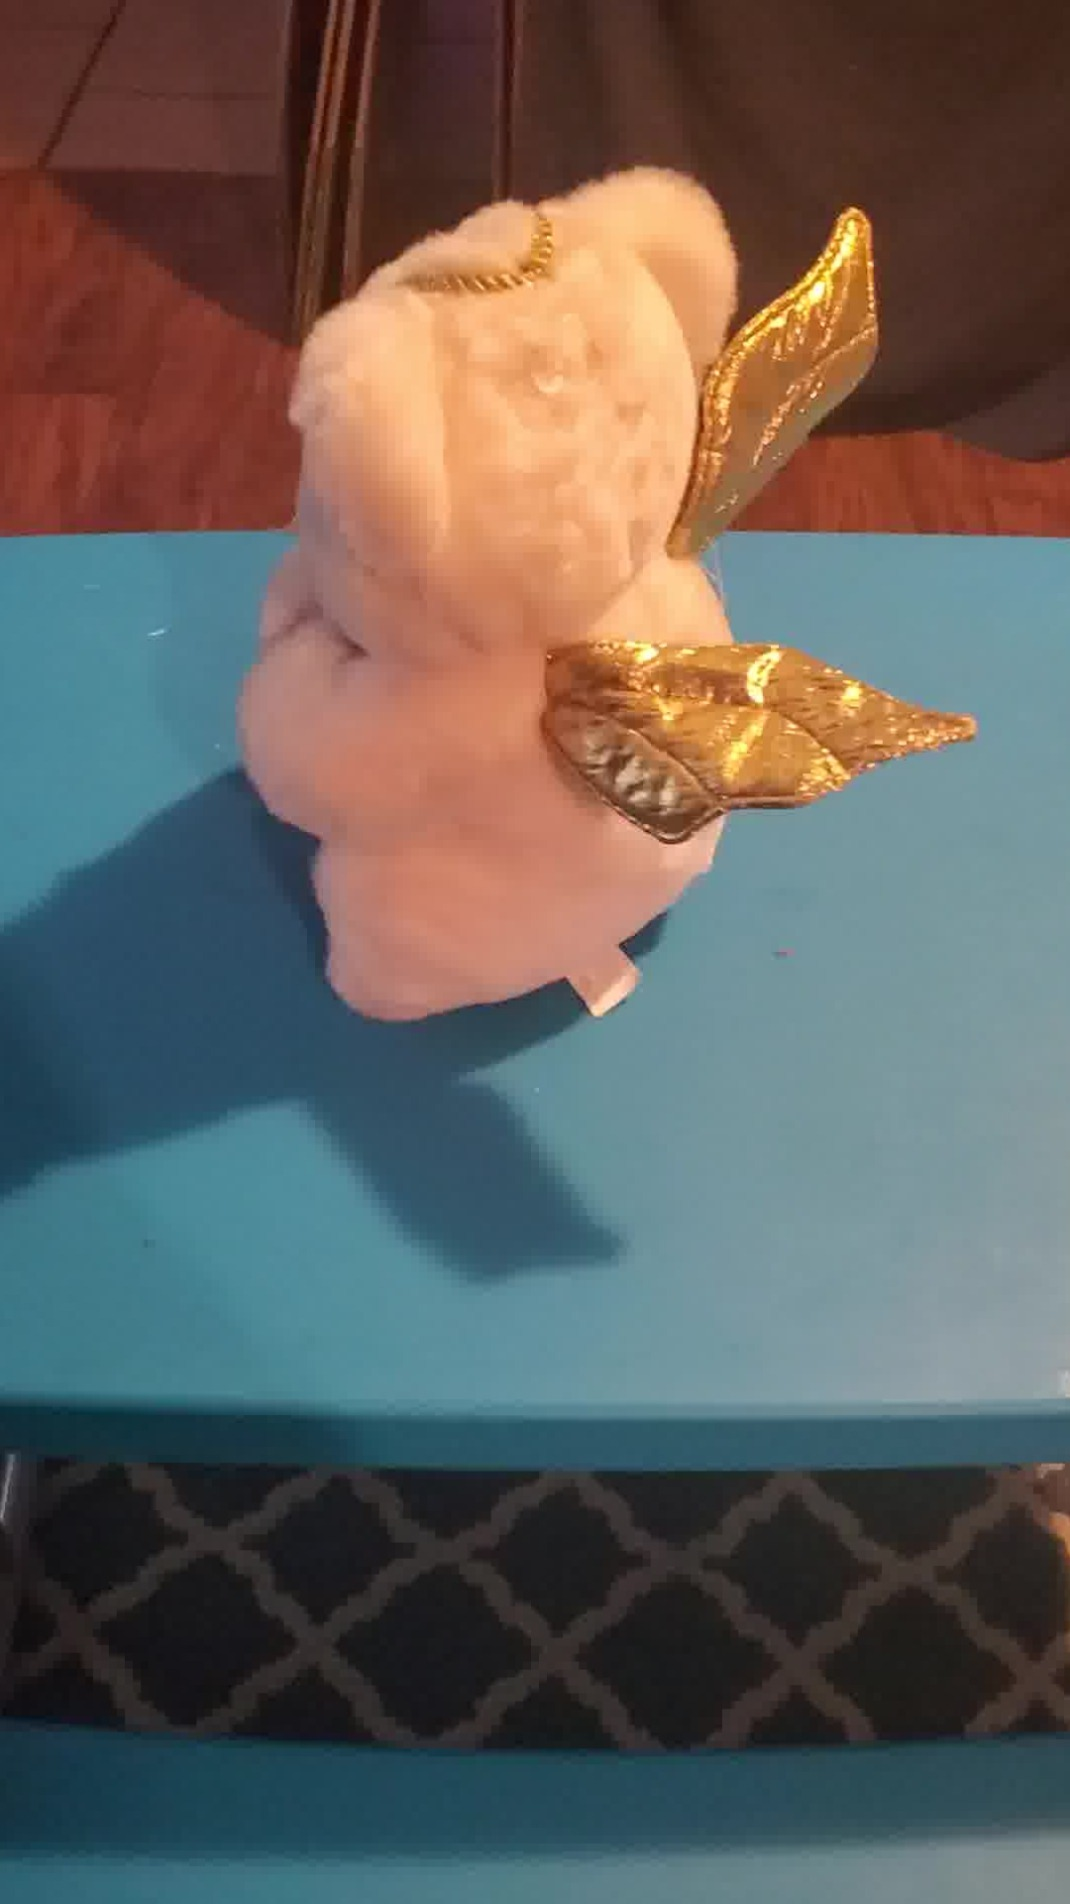
\includegraphics[width=\linewidth]{figures/sample_object/view_02.jpg}
        \vspace{2mm}
        \texttt{view\_02}
    \end{minipage}
    \hfill
    \begin{minipage}{0.18\textwidth}
        \centering
        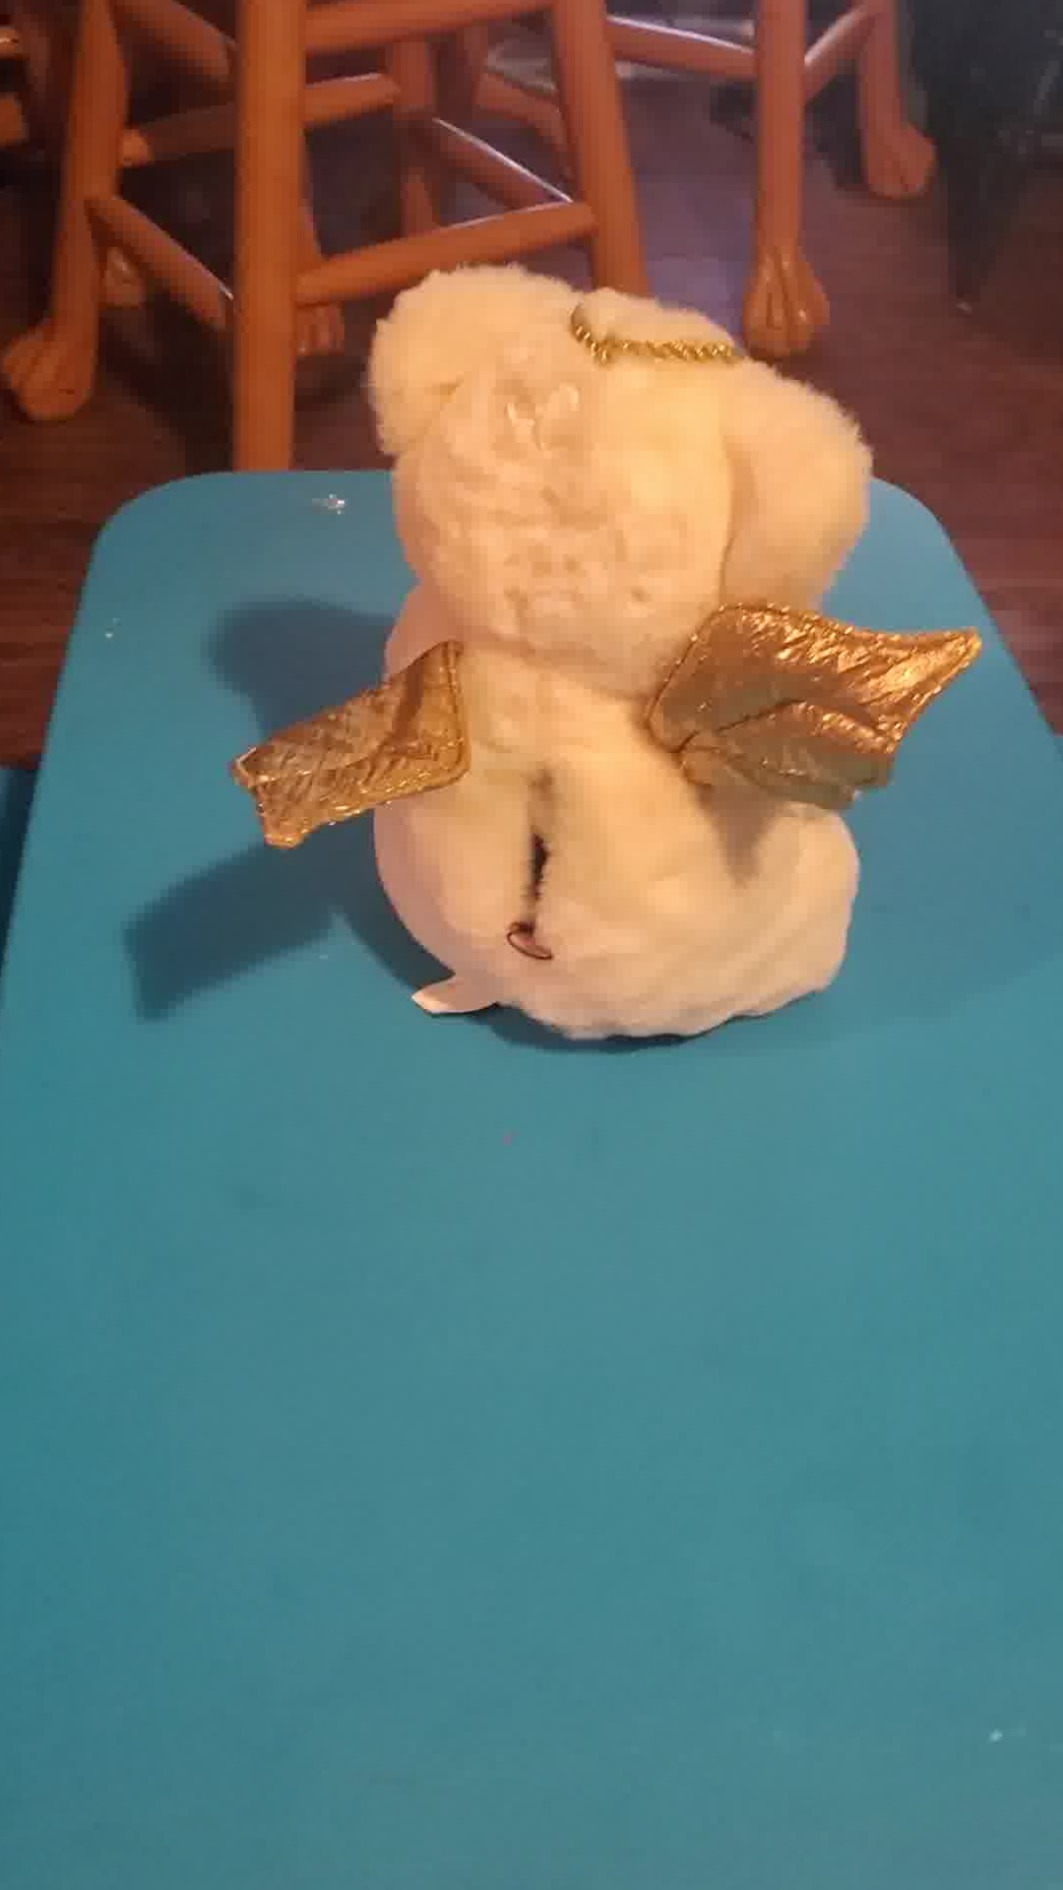
\includegraphics[width=\linewidth]{figures/sample_object/view_03.jpg}
        \vspace{2mm}
        \texttt{view\_03}
    \end{minipage}
    \hfill
    \begin{minipage}{0.18\textwidth}
        \centering
        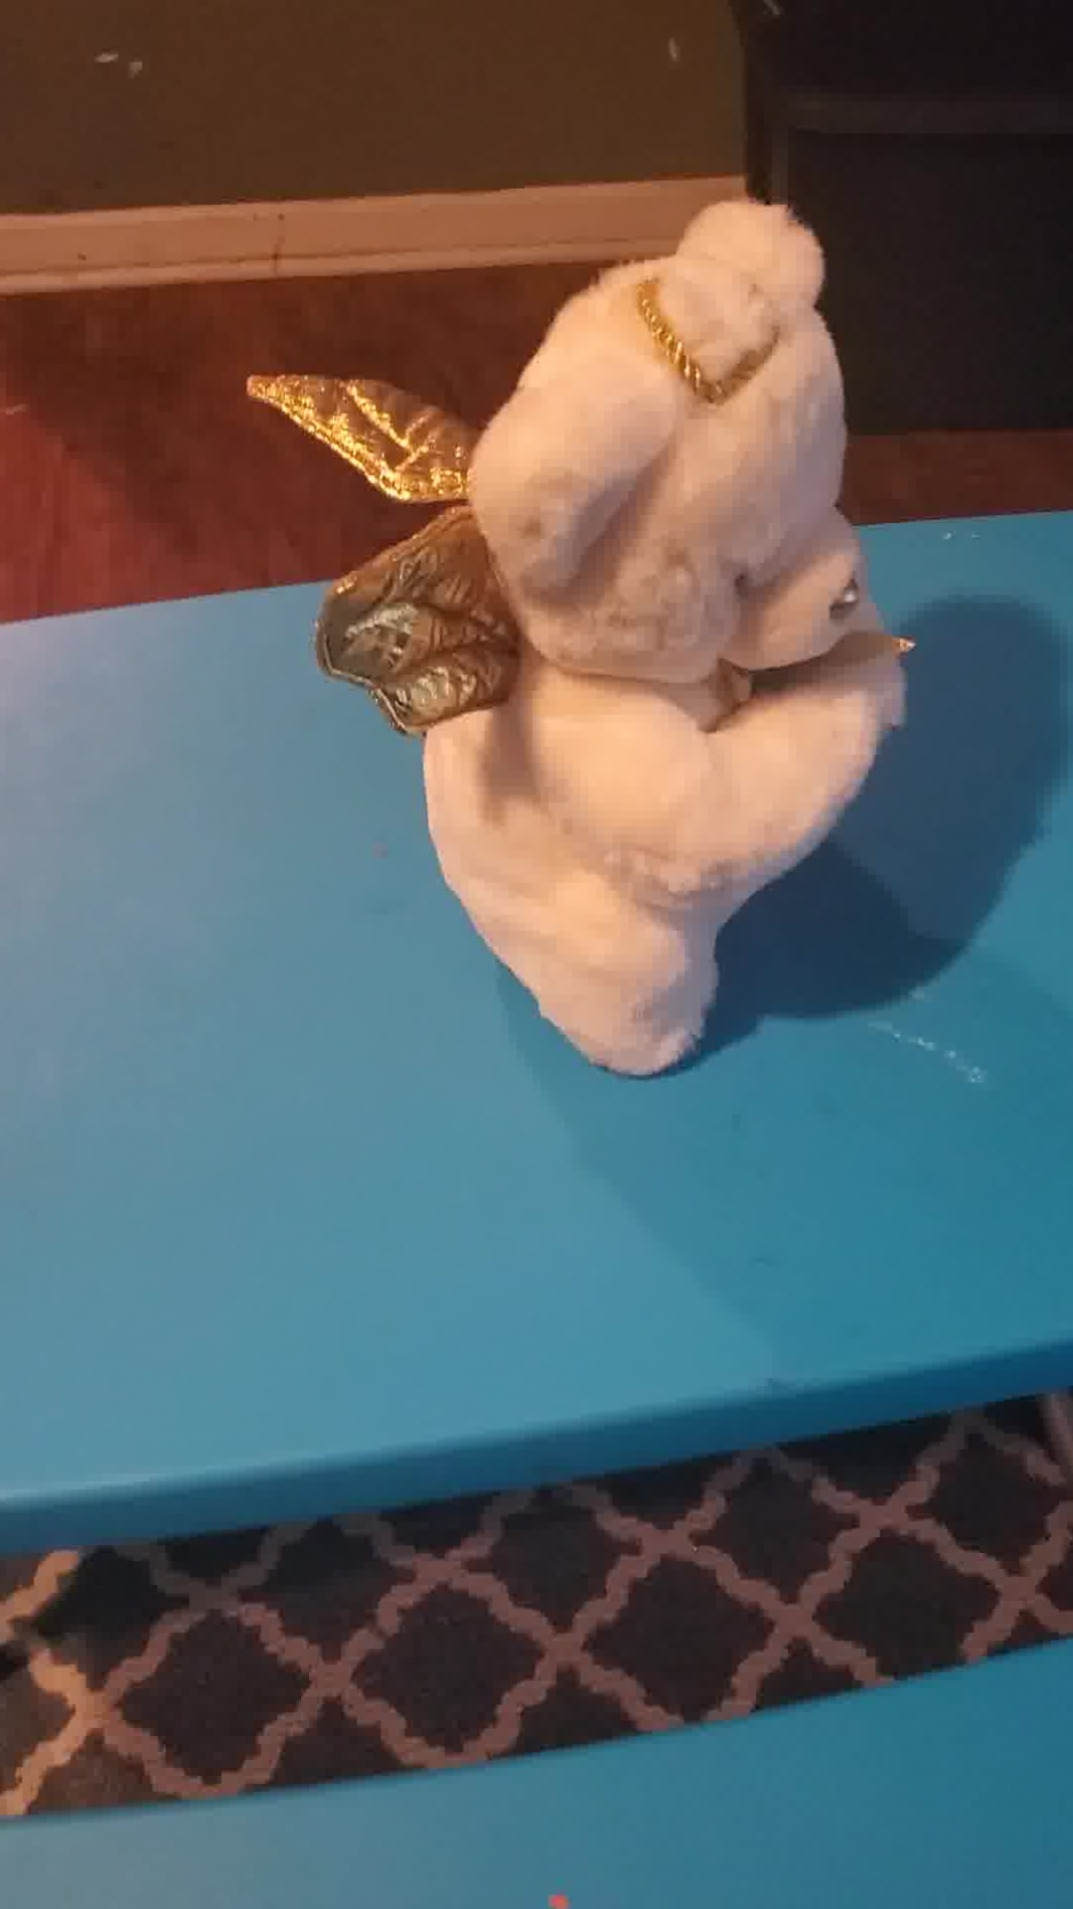
\includegraphics[width=\linewidth]{figures/sample_object/view_04.jpg}
        \vspace{2mm}
        \texttt{view\_04}
    \end{minipage}
    \hfill
    \begin{minipage}{0.18\textwidth}
        \centering
        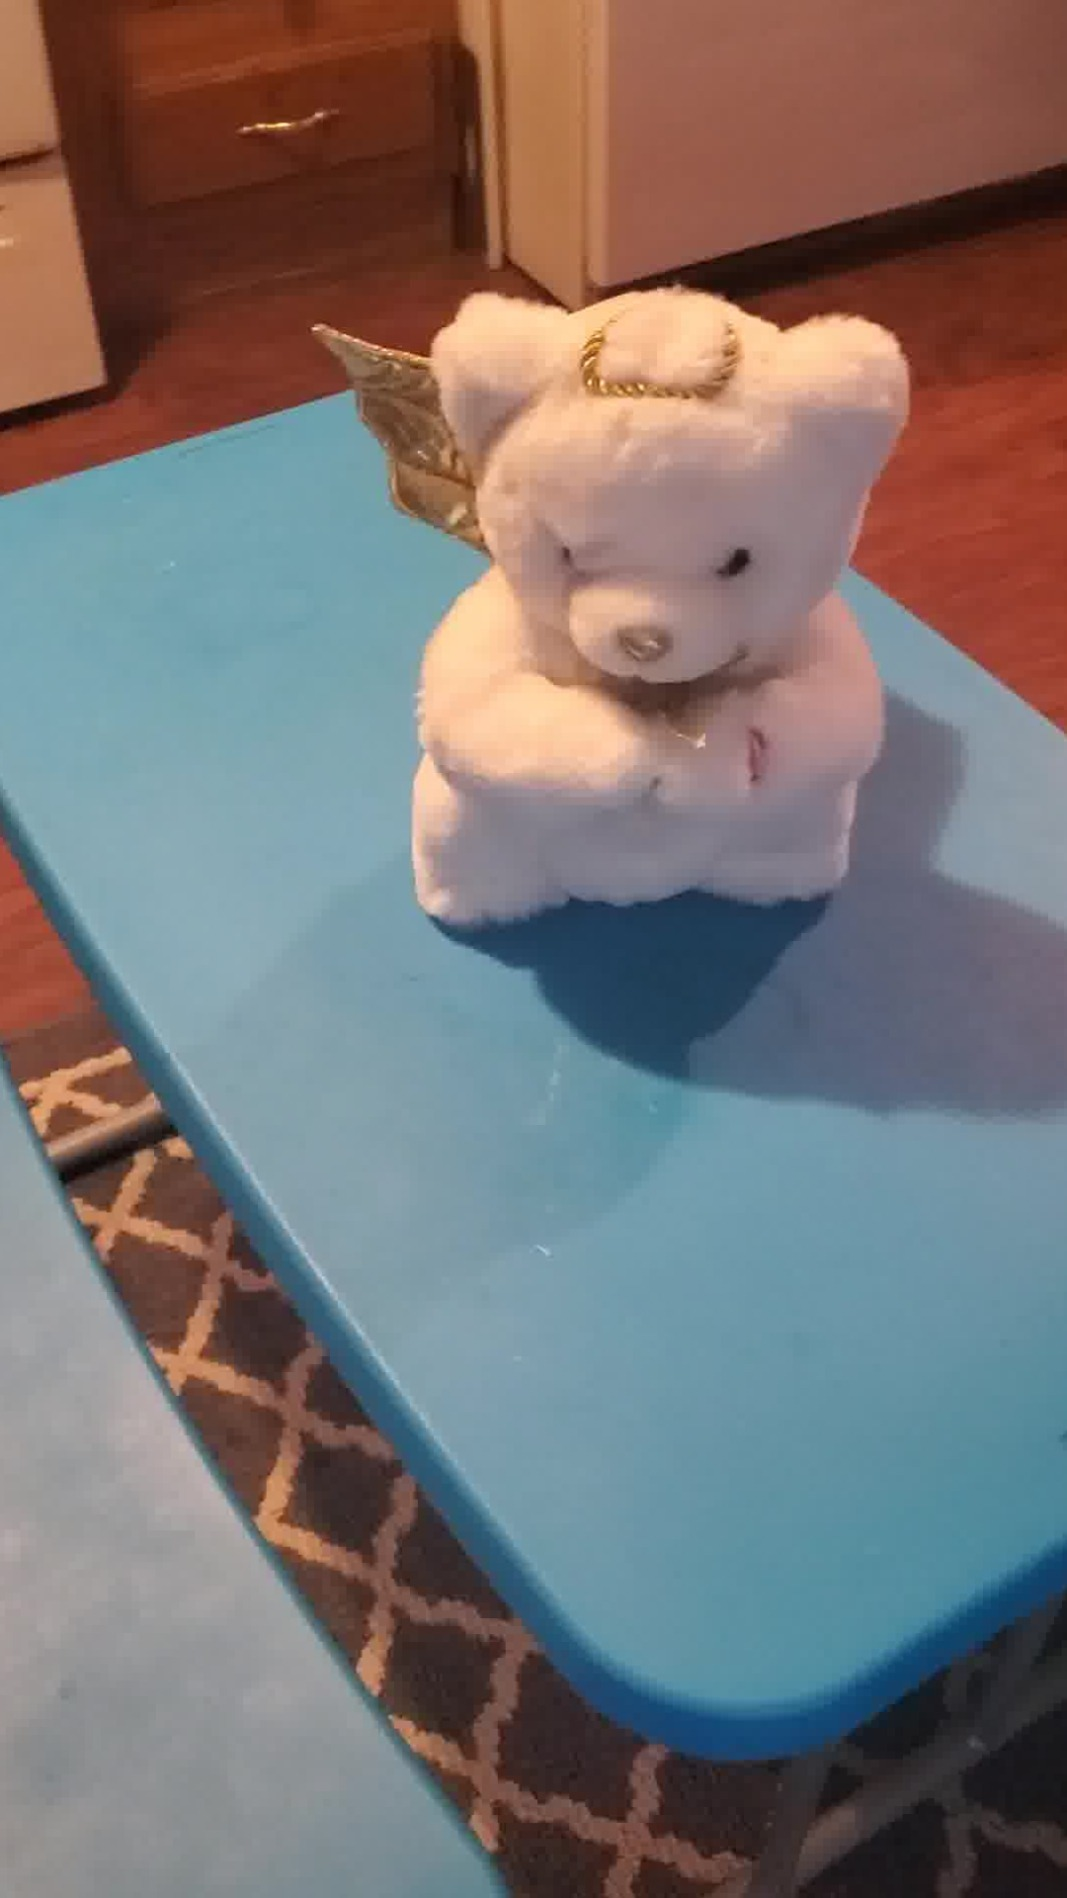
\includegraphics[width=\linewidth]{figures/sample_object/view_05.jpg}
        \vspace{2mm}
        \texttt{view\_05}
    \end{minipage}

    \caption{Example of five candidate viewpoints for one object instance.}
    \label{fig:sample-five-views}
\end{figure}

\section{Sample UMD Annotation Entry}

Table~\ref{tab:sample-umd-entry} shows an example UMD-derived sample.

\begin{table}[htbp]
    \centering
    \caption{Sample UMD+GT-derived annotation entry.}
    \label{tab:sample-umd-entry}
    \begin{tabular}{ll}
        \hline
        Field & Example \\
        \hline
        Tool / category & \texttt{mug\_01} / \texttt{mug} \\
        Affordance & \texttt{grasp} \\
        Instruction & \textit{find the view of the mug where the handle} \\
         & \textit{is most clearly visible for grasping} \\
        Split & \texttt{test} \\
        GT rule & affordance area \(\geq 0.8 \times \max\) area \\
        \hline
    \end{tabular}
\end{table}
